\section*{Mutagenesi \emph{in vitro}}

	\subsection*{Indroduzione}
        Nella prima esperienza si vuole verificare l'efficacia e la precisione della polimerasi in presenza di sostanze tossiche e/o inibitorie.
        L'organismo modello utilizzato è stato il lievito Saccharomyces Cerevisiae in forma aploide.
	Viene utilizzata come sostanza inibitoria il cloruro di manganese \emph{$MnCl_2$}.
	Il DNA prodotto verr\`a poi visualizzato attravero \emph{PCR} ed elettroforesi.
        
		\subsubsection*{Polimerase chain reaction \emph{PCR}}
		In vitro viene utilizzato il calore per separare le due eliche di DNA mentre in natura questo compito è affidato a un enzima elicasi. 
       		 Si abbassa poi la temperatura per far legare il primer a una sequenza precisa per permettere alla PCR di trovare un 3'-OH da cui iniziare la replicazione.
        	Questo processo verrà ripetuto più volte.

		\subsubsection*{Effetti del cloruro di manganese}
        	Gli ioni magnesio sono usati come catalizzatori della polimerizzazione favorendo la sostituzione nucleofilica del 3'-OH libero del primer con il fosfato del nucleotide.
        	Il manganese può competere con il magnesio per l'accesso al sito allosterico? Se si, può cambiarne l'efficienza?
        	Proveremo a rispondere aggiungendo alla reazione di PCR cloruro di manganese.

		\subsubsection*{DNA da amplificare}
        	La sequenza di DNA da amplificare inoltre non sarà scelta a caso, ma sarà la sequenza che codifica per un gene reporter.
		Nella cellula verrà inserito anche un plasmide linearizzato, pRDI22, che dovrà avere un'origine di replicazione riconoscibile dall'organismo ospitante e una regione centromerica, in modo da poter essere scambiato per un plasmide del lievito.
        	Il plasmide conterrà il gene reporter, per conferirgli la capacità di essere replicato all'interno della cellula, e il gene leu, per cui il ceppo di lievito utilizzato è auxotrofo, questo permetterà di selezionarlo.
        	Oltre all'auxotrofia per la leucina, che servirà a verificare l'efficacia di pRDI22, il ceppo utilizzato sarà auxotrofo per l'adenina, in questo modo, si può verificare il funzionamento di P53.

	\subsection*{Risultati attesi}
	L'esperimento si propone di osservare l'effetto del manganese sulla replicazione, in particolare:
	\begin{itemize}
		\item Se il manganese pu\`o influenzare i risultati della \emph{PCR}.
       		\item Se il manganese pu\`o introdurre mutazioni.
	\end{itemize}
	Trasformando cellule con il risultato della \emph{PCR} si verifica la funzionalit\`a del gene amplificato.
        Se il gene reporter è replicato in maniera corretta, i lieviti con questo gene cresceranno di colore bianco, se il DNA viene mutato, il lievito crescerà con colorazione tra il rosso e il rosato.

   	\subsection*{Risultati}
        Sono state usate quattro diverse concentrazioni di manganese cloruro, $0M$, $0.25M$, $0.5M$ e $1M$, più una provetta di controllo negativo senza DNA per verificare la purezza dei reagenti.
	\begin{figure}[H]
		\centering
		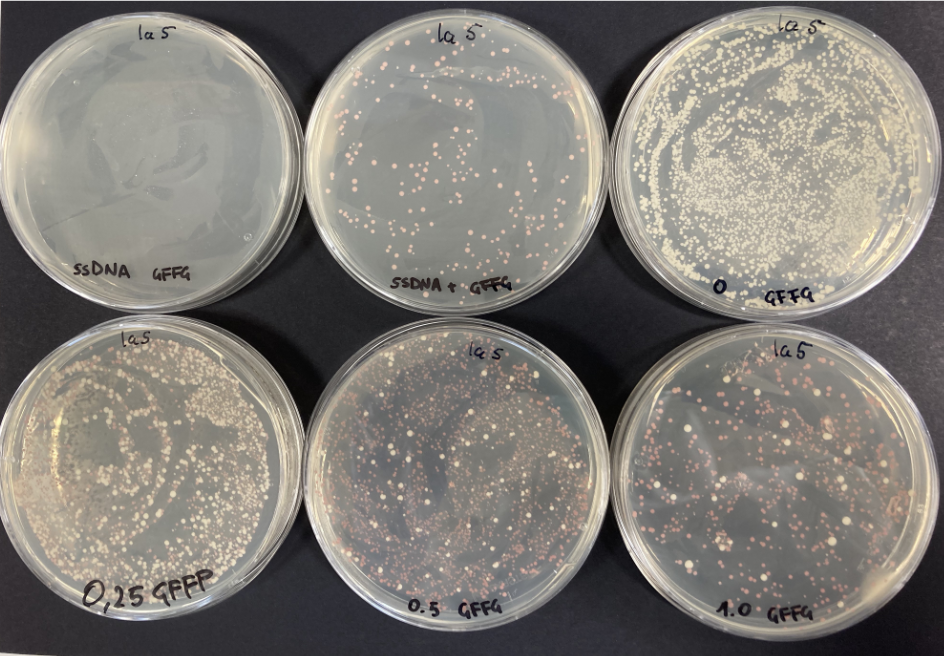
\includegraphics[scale=0.4]{./Pics/MutVitro/Contebatteriche.png}
		\caption{Colonie formatesi a diverse concentrazioni di \emph{$MnCl_2$}}
		\label{fig1}
	\end{figure}

	\begin{table}[H]
		\centering
		\begin{tabular}{|c|c|c|c|c|}
			\hline
			\makecell{Concentrazione di \emph{$MnCl_2$}} & $0M$ & $0.25M$ & $0.5M$ & $1M$\\
			\hline
			\makecell{Conta totale} & $2672CFU$ & $1822CFU$ & $1778CFU$ & $599CFU$ \\
			\hline
			\makecell{Colonie mutate} & $236CFU$ & $1044CFU$ & $1672CFU$ & $5564CFU$\\
			\hline
			\makecell{Tasso di mutazione} & $8.83\%$ & $57.3\%$ & $94\%$ & $94.16\%$\\
			\hline
		\end{tabular}
		\caption{Conta delle colonie}
		\label{tab}
	\end{table}

	\subsection*{Considerazioni finali}
	I risultati ottenuti, come si vede nella tabella~\ref{tab}, dimostrano come, non solo il cloruro di manganese riesca a competere con il magnesio per l'accesso al sito allosterico,
        ma anche quanto riesca a influire sia sull'efficienza della replicazione, che sulla sua precisione.
        Al crescere della concentrazione di manganese cloruro infatti, la conta totale di cellule in piastra, diminuisce, mentre aumenta la percentuale delle cellule mutate.
        (La presenza di un certo tasso di mutazione anche nella soluzione senza manganese è imputabile all'affidabilità della PCR stessa).
